\documentclass{acm_proc_article-sp}

\usepackage{graphicx}
\usepackage{hyperref}

\usepackage{framed}

\newenvironment{cframed}[1][blue]
  {\def\FrameCommand{\fboxsep=\FrameSep\fcolorbox{#1}{white}}%
    \MakeFramed {\advance\hsize-\width \FrameRestore}}
  {\endMakeFramed}

\usepackage{xcolor}         % colors
\definecolor{scarlet}{HTML}{FF2400}

%% \documentclass{article}
%% \usepackage[sc]{mathpazo}
%% \usepackage[T1]{fontenc}
%% \linespread{1.05} % Palatino needs more space between lines
%% \usepackage{microtype}
%% \usepackage[hmarginratio=1:1,top=32mm,columnsep=20pt]{geometry}
%% \usepackage{graphicx}
%% \usepackage{hyperref}
%% \usepackage{framed}
%% \newenvironment{cframed}[1][blue]
%%   {\def\FrameCommand{\fboxsep=\FrameSep\fcolorbox{#1}{white}}%
%%     \MakeFramed {\advance\hsize-\width \FrameRestore}}
%%   {\endMakeFramed}
%% \usepackage{xcolor}         % colors
%% \definecolor{scarlet}{HTML}{FF2400}
%% \usepackage{multicol}

\begin{document}

\title{Roadmaps in Peer Learning}


\numberofauthors{6} %  in this sample file, there are a *total*
% of EIGHT authors. SIX appear on the 'first-page' (for formatting
% reasons) and the remaining two appear in the \additionalauthors section.
%
\author{
% You can go ahead and credit any number of authors here,
% e.g. one 'row of three' or two rows (consisting of one row of three
% and a second row of one, two or three).
%
% The command \alignauthor (no curly braces needed) should
% precede each author name, affiliation/snail-mail address and
% e-mail address. Additionally, tag each line of
% affiliation/address with \affaddr, and tag the
% e-mail address with \email.
%
% 1st. author
\alignauthor
Joseph Corneli\\
\affaddr{Knowledge Media Institute}\\
\affaddr{The Open University}\\
\affaddr{Milton Keynes, UK}\\
\email{joseph.corneli@open.ac.uk}
% 2nd. author
\alignauthor
Charles Jeffrey Danoff\\
\affaddr{Mr Danoff's Teaching Laboratory}\\
\affaddr{Chicago, IL}\\
\email{charles@danoff.org}
% 3rd. author
\alignauthor
Fabrizio Terzi \\
\affaddr{Bergamo HUB}\\
\affaddr{Bergamo, IT}\\
\email{fabrizio.terzi@gmail.com}
\and  % use '\and' if you need 'another row' of author names
% 4th. author
\alignauthor Charlotte Pierce \\
\affaddr{Pierce Press} \\
\affaddr{Arlington, MA}\\
\email{charlotte.pierce@gmail.com}
% 5th. author
\alignauthor John Graves \\
\affaddr{Auckland University of Technology}\\
\affaddr{Auckland, NZ}\\
\email{jgraves@aut.ac.nz}
% 6th. author
\alignauthor R\'egis Barondeau \\
\affaddr{Universit\'e du Qu\'ebec \`a Montr\'eal}\\
\email{regis.barondeau@mac.com}
}

% There's nothing stopping you putting the seventh, eighth, etc.
% author on the opening page (as the 'third row') but we ask,
% for aesthetic reasons that you place these 'additional authors'
% in the \additional authors block, viz.
% \additionalauthors{Additional authors: John Smith (The Th{\o}rv{\"a}ld Group,
% email: {\texttt{jsmith@affiliation.org}}) and Julius P.~Kumquat
% (The Kumquat Consortium, email: {\texttt{jpkumquat@consortium.net}}).}
% \date{30 July 1999}

% Just remember to make sure that the TOTAL number of authors
% is the number that will appear on the first page PLUS the
% number that will appear in the \additionalauthors section.


\maketitle
\begin{abstract}

Following a year of productive learning and work culminating in the first edition of The Peeragogy Handbook we reflect here on lessons learned and patterns uncovered. In the second half of the paper we outline our goal: to transition from an innovative theoretical project to a sustainable, easily replicable peer project problem solving accelerator.

\end{abstract}


%%%%%%%%%%%%%%%%%%%%%%%%%%%%%%%%%%%%%%%%%%%%%%%%%%%%%%%%%%%%%%%%%%%%%%%%%%%%%%%%%%%%%% Cut here

\section{The Peeragogy Project}

The Peeragogy project is a group of adult learners trying to uncover
the most effective ways to do collaborative learning. We have been
working together in an open online community since January, 2012.

Our methodology is based on examining and recording how we learn and
work together, and on existing examples and theories of peer learning.
We encourage participants to build and share experiments and case
studies, e.g. the classroom intervention ``5PH1NX''\footnote{\url{http://peeragogy.org/case-study-5ph1nx/}}, the virtual
development collaboration hosted by the Free Technology Guild\footnote{\url{http://campus.ftacademy.org/wiki/index.php/Main_Page}}, the new
Bergamo Hub\footnote{\url{http://paragogy.net/Bergamo_HUB:_il_potere_di_innovare_attraverso_la_collaborazione}}, a civic center and maker space.
We have encouraged participants to share and critically reflecting on their own learning projects, to augment our own reflection on Peeragogy principles and features. In this way, the Peeragogy project has increasingly come to serve as a distributed, research-based, project incubator.

This paper describes the qualitative aspects of participation in this
project. Our findings can be used by other projects with a
collaborative focus, and serve as a ``humanities-friendly'' accompaniment to
previous writing about collaboration in open source software
(\cite{OpenAdvice}, \cite{crowstonXdefiningX2003}).  We have a learning focus that is missing from other more general discussions of online community \cite{bacon2012art}.

One of the key features we will attempt to convey in this paper is the multiplicity of possible narratives.  That is to say, each participant in the project has a different view of what it is about, how it is useful for them, and \emph{how} useful it is for others, and this is also true for the authors of the current paper. The motivations reported by participants in the Peeragogy project include:
\begin{itemize}
\item Acquisition of training or support in a topic or field;
\item Building relationships with interesting people;
\item Finding professional opportunities through other participants;
\item Creating or bolstering a personal network;
\item More organized and rational thinking through dialog and debate; and
\item Feedback about their own performance and understanding of the
  topic.
\end{itemize}

Each of those motivations can affect the vitality of the Peeragogical process and the end result for the individual participant. Person-specific motivations are also met by person-specific obstacles. In addition to reports from our own experiences with the project, this paper draws on qualitative survey data to bring in the voices and views of other authors, readers, and discussants ($N=250$, $RR=17\%$).

\section{Acknowledgements}

The Peeragogy project was instigated by Howard Rheingold, adapting Corneli and Danoff's \cite{paragogy} work on Paragogy to build a
less-academic, more practical, DIY Handbook for peer learning by assembling a group of contributors that included, in addition to the current authors: Bryan Alexander, Paul Allison, Doug Breitbart, Suz Burroughs, Jay Cross, Julian Elve, Mar\'ia Fernanda, James Folkestad, Kathy Gill, Gigi Johnson, Anna Keune, Roland Legrand, Christopher Neal, Ted Newcomb, Stephanie Parker, David Preston, Paola Ricaurte, Stephanie Schipper, and Geoff Walker.

\begin{figure}
\begin{center}
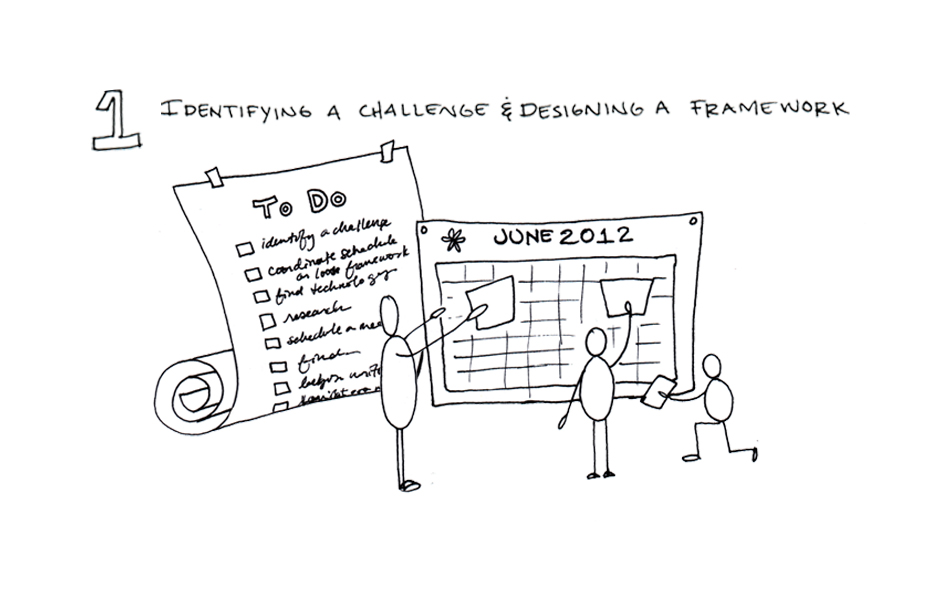
\includegraphics[width=.5\textwidth]{OpenBook1.jpg}
\vspace{-.7in}
\end{center}
\caption{Work by Amanda Lyons on ``Peeragogy in Action''
  \cite{PeeragogyinAction} \label{amanda}}
\end{figure}

\section{Methodology}

The paper is essentially an experience report supplemented by qualitative survey data. These methods seem suitable for phenomenological research that focuses on the question: ``what is it like to participate in the Peeragogy project?''. For Patton\cite{patton}, to gather phenomenological data: 
\begin{quote}
"one must undertake in-depth interviews with people who have direcly experienced the phenomenon of interest; that is, they have "lived experience" as opposed to secondhand experience"
\end{quote}

While we did not do in-depth intreviews, some of these reflections will generalize to other peer learning projects, and Section \ref{accelerator} provides examples.

We have drawn on the ``research through writing'' method pioneered by Tomlinson \emph{et al.} \cite{tomlinson2012massively}, with reference to earlier work by Christopher Frayling on ``research through design'' \cite{frayling1993research}. There is also a significant design aspect to the project -- effectively ``design through practice''. Indeed, as Frayling remarked: ``Research is a practice, writing is a practice, doing science is a practice, doing design is a practice, making art is a practice.''

At the core of both this paper (Section \ref{patterns}) and the Peeragogy Handbook (Chapter III) are a set of Alexandrian patterns that describe the practice of Peeragogy. These patterns developed through observation of the Peeragogy project from its initial days, and through discussion and debate among the current authors.

\section{The Peeragogy Handbook}

Peeragogy is a set of replicable techniques and patterns for effective
peer learning and problem solving.  Evidence that this can work comes
from our project: without the support of a unifying formal
institution, over the course of one year, a group of volunteers came
together and wrote a cohesive treatise, The Peeragogy Handbook, that is far richer
than what any one of them might have produced working alone.

We utilized a variety of technologies to write the book: live
meetings and a loose bureaucracy of teams and team leaders for
different sub-projects. We elected to use the Creative Commons Zero
Public Domain Dedication for all of our work, to maximize its
potential for re-use. Contributors submitted texts, images, and
videos, and in addition to our handbook, we prepared several external
presentations and publications (cf. Figure \ref{amanda}).

We used a blend of synchronous and asynchronous collaboration, and a
whole suite of tools: the Social Media Classroom (a multi-purpose platform based on Drupal 6) [SMC], Diigo, Google Docs, Google+, WordPress, LaTeX, Lulu, Twitter, Blackboard Collaborate, Git, Google Hangouts, Mumble, and more.

Each of these tools has its own pros and cons and fits a certain
purpose -- Peeragogy is not bound to particular digital tools nor the
digital world at all. For example, a physical interpretation was
given to the project by Anna Keune, Paola Ricaurte, Gigi Johnson and Amanda Lyons who held a
workshop at the Open Knowledge Conference 2012 in Helsinki\footnote{
  \url{http://okfestival.org/peeragogy-handbook-workshop/} and
  \url{http://www.youtube.com/watch?v=P2UJrN58MVI}, leading to the
  Peeragogy contribution to the Open Book \cite{PeeragogyinAction}.},
and also with the work-in-progress by Fabrizio Terzi to build a peer learning focused community center.

Intuitively, there are bound to be difficulties for a group of peers studying a subject together, outside a traditional classroom or without a teacher. Indeed, peer learning is different from other forms of group effort, the proverbial ``barnraising'' for example, in which the persons involved can be presumed to know how to build barns - or at least to know someone who knows, and stand ready to take orders. Typically, peers are not experts in learning, didactics, or in the subject they are studying, and are faced with multiple difficulties associated with putting together knowledge about the subject, assembling a suitable learning strategy, and communicating with one another \cite{paragogy}. In addition to these \emph{a priori} barriers, we needed to create achievable common goals and overcome differences in timezone, language fluency, experience with technology, writing, learning, and engagement styles.

Our strategy focused on using use each participant's differences as
points of strength. In essence, we have high cognitive diversity, and, since we all roughly agree about what we are
aiming for in the project we have allowed ourselves to be
inspired by one another. We experiment often with new tools; however, the project has three main ``hubs'':
the Social Media Classroom, where we started writing, the Wordpress
site peeragogy.org, where we host the master copy of the handbook, and
our Google+ community. Each new tool and contribution poses questions
about how to connect back to the overall flow of work and the book
outline.

At a high level, the goal of producing a handbook explaining how other
peers could learn effectively with other peers on a given project kept
things cohesive, and gave us a standard of quality.  Producing the
book proved to be a viable method for researching and deepening our
understanding of peer learning.

Version 1.0 of the Peeragogy Handbook presents a range of techniques
that self-motivated learners can use to connect with each other and
develop stronger communities and collaborations. We are continuing to
refine the book in the open, and we aim to publish Version 2.0 on
January 1, 2014.

In the mean time, we are also building on what we learned to
transition from an innovative theory-driven research project to a
sustainable and replicable peer produced problem solving accelerator.

\subsection{What we learned}

We have identified several basic and more elaborated patterns (in the
sense of \cite{Origins}, \cite{Tales}, \cite{vlissides1995design})
that describe ``the Peeragogy effect''.  The central pattern is that
of a Roadmap, which can apply at the individual level, as a personal
learning plan, or at a project level.\footnote{See ``What are Learning
  Analytics?'' by George Siemens
  \url{http://www.elearnspace.org/blog/2010/08/25/what-are-learning-analytics/}
  for more on individual learner profiles as a context for developing
  and tracing progress on individual learning plans.} The roadmap may
include a reason ``why'' \cite{sinek2009start}, exposition about the
goal, indicators of progress, a section for future work, and so forth.
Our initial roadmap for the project was the preliminaly outline of the
handbook; as the handbook approached completion, we spun off
additional goals into a new roadmap for developing further aspects of
the project.\footnote{\url{http://peeragogy.org/peeragogy-org-roadmap/}}. Group culture around maintaining and updating the roadmap define
project governance. Other patterns flesh out the project's properties in a sort of ``agora'' of possibilities.

\subsection{Patterns} \label{patterns}

Thus far the following patterns have emerged:

\vspace{.2in}
\hspace{.2in}
\begin{minipage}{.4\textwidth}
\begin{description}
\item[Roadmap] Plans for future work, direction towards a goal, dynamic.
\item[Convene] \quad \\[-.1in]
\begin{itemize}
\item[\emph{Project}] Most projects involve learning.
\item[\emph{Guide}] Overviews expose the lay of the land collecting content
  and stories.
\end{itemize}
\end{description}
\end{minipage}

\hspace{.2in}
\begin{minipage}{.4\textwidth}
\begin{description}
\item[Organize] \quad \\[-.1in]
\begin{itemize}
\item[\emph{Roles}] Specialize and mix it up. Play to participants' strengths and skills.
\item[\emph{Newcomer}] Create a guide for ``beginner's mind'' and help avoid
  need to bring new members up to speed each ``meeting.''
\item[\emph{Wrapper}] Consolidate and contain. Front end appearance to
  participants.
\end{itemize}
\end{description}
\end{minipage}

\hspace{.2in}
\begin{minipage}{.4\textwidth}
\begin{description}
\item[Cooperate] \quad \\[-.1in]
\begin{itemize}
\item[\emph{Heartbeat}] The ``heartbeat'' of the group keeps energy flowing.
\item[\emph{Capacity}] Know your limits, find ways to get other people
  involved.
\item[\emph{Moderation}] When leaders step back, dynamics can improve;
  moderator serves as champion and editor.
\item[\emph{Poll}] Invite brainstorming, collecting ideas, questions, and
  solutions.
\item[\emph{Patience}] Do not hold grudges and do not make pithy comments
  about team members or other institutions.
\end{itemize}
\end{description}
\end{minipage}

\hspace{.2in}
\begin{minipage}{.4\textwidth}
\begin{description}
\item[Assess]  \quad \\[-.1in]
\begin{itemize}
\item[\emph{Reuse}] Repurposing, tinkering, or creating from scratch?
\item[\emph{Discern}] Found a pattern? Give it a title and example.
\item[\emph{Believe}] Participants need to buy in to the idea or philosophy behind a project.
\item[\emph{Sacrifice}] Participants must be willing to sacrficice credit.
\end{itemize}
\end{description}
\end{minipage}

These patterns provide a natural framework for participatory design
and research in peer learning projects.  For example, can use them to
provide a terse profile for our project (Figure \ref{catalog}).

\begin{figure}[h]
\begin{cframed}[black]
{\bf Roadmap}: We aim to build a Wikipedia style project for
learning. After developing a learning resource for a year, our handbook toolbox can now serve as an accelerator for other peer learning projects. As that happens those projects will feedback into the handbook itself making it more useful. \\

\emph{Guide}: The Handbook is our guide for ourselves and newcomers. \\

\emph{Wrapper}: Our wrapper provided weekly or
bi-weekly summaries throughout the duration of the project. \\

\emph{Heartbeat}: Multiple peers hosted live meetings using Google Hangouts or BlackBoard Collaborate. \\

\emph{Capacity}: The SMC forum is accessible only to logged in
users. We have also made routine efforts to ``prune'' the list of
contributors by asking people to actively renew interest or leave.
This gives us a core group of active contributors. \\

\emph{Poll}: Google+ has been a place to bring in new ideas and links to other projects. \\

\emph{Reuse}: We have not had to build any special-purpose software to
run the project.  \\

\emph{Believe}: We have worked hard to make it easy for people to ``convert''
into contributors; there is qualitatively a missionizing aspect to the
project, and we have drawn on previous work in this space to refine
our approach, particularly with regard to the efficiency of bringing
in groups rather than individuals \cite{Bridges}.
\end{cframed}
\vspace{-.2in}
\caption{Terse description of the Peeragogy project using our pattern catalog \label{catalog}}
\end{figure}

\subsection{Survey} \label{survey}

In an effort to document "the paths in the grass" \cite{Wall} that come from unexpected links between different things in our successful publication of The Peeragogy Handbook we prepared a short survey for Peeragogy project participants. We asked people how they had participated (e.g., Signing up for access to the Social Media Classroom and mailing list, Joining the Google+ Community, Authoring articles, etc.), and what goals or interests motivated their participation. We asked them to describe the Peeragogy project itself in terms of its aims and to evaluate its progress over the first year of its existence. As another measure of ``investment'' in the project, we asked, with no strings attached, whether the respondent would consider donating to the Peeragogy project. This survey was circulated to 223 members of the Peeragogy Google+ community, as well as to the currently active members of the Peeragogy mailing list.

The outline of the project's purpose ranged from the general: ``How to
make sense of learning in our complex times'' - to much more
specific:

\begin{quote}
``Push education further, providing a toolbox and [techniques] to
self-learners. In the peeragogy.org introduction page we assume that
self-learners are self-motivated, that may be right but the Handbook
can also help them to stay motivated, to motivated others and to face obstacles that may erode motivation.''
\end{quote}

Considering motivation as a key factor, it is interesting to observe
how various understandings of the project's aims and its flaws
intersected with personal motivations. For example, one respondent
(who had only participated by joining the Google+ community) was:
``[Seeking] [i]nformation on how to create and engage communities of
interest with a shared aim of learning."

More active participants justified their participation in terms of what they get out of taking an active role, for instance:

\begin{quote}
``Contributing to the project allows me to co-learn, share and co-write ideas with a colourful mix of great minds. Those ideas can be related to many fields, from communication, to technology, to psychology, to sociology, and more.''
\end{quote}

The most active participants justified their participation in terms of
beliefs or a sense of mission:

\begin{quote}
``Currently we are witnessing many efforts to incorporate technology as
an important tool for the learning process. However, most of the
initiatives are reduced to the technical aspect (apps, tools, social
networks) without any theoretical or epistemological
framework. Peeragogy is rooted in many theories of cooperation and
leads to a deeper level of understanding about the role of technology
in the learning process. I am convinced of the social nature of
learning, so I participate in the project to learn and find new
strategies to learn better with my students.''
\end{quote}

Or again:

\begin{quote}
``I wanted to understand how "peer production" really works. Could we
create a well-articulated system that helps people interested in peer
production get their own goals accomplished, and that itself grows and
learns? Peer production seems linked to learning and sharing - so I
wanted to understand how that works.''
\end{quote}

They also expressed criticism of the project, implying that they may feel rather powerless to make the changes that would correct course:

\begin{quote}
``Sometimes I wonder whether the project is not too much `by education specialists for education specialists'. I have the feeling peer learning is happening anyway, and that teens are often amazingly good at it. Do they need `learning experts' or `books by learning experts' at all? Maybe they are the experts. Or at least, quite a few of them are.''
\end{quote}

Another respondent was more blunt:

\begin{quote}
``What problems do you feel we are aiming to solve in the Peeragogy
project? We seem to not be sure. How much progress did we make in the
first year? Some..got stuck in theory.''
\end{quote}

But, again, it is not entirely clear how the project provides clear pathways for contributors to turn their frustrations into changed behavior or results. Additionally we need to be entirely clear that we are indeed paving new ground with our work. If there are proven peer learning methods out there we have not examined and included in our efforts, we need to find and address them. Peeragogy is not about reinventing the wheel.

It is also not entirely clear whether excited new peers will find pathways to turn their excitement into shared products or process. For example, one respondent (who had only joined the Google+ community) had not yet introduced their fascinating projects publicly:

\begin{quote}
``I joined the Google+ community because I am interested in developing peer to peer environments for my students to learn in. We are moving towards a community-based, place-based program where we partner with community orgs like our history museum for microhistory work, our local watershed community and farmer's markets for local environmental and food issues, etc. I would love for those local efforts working with adult mentors to combine with a peer network of other HS students in some kind of cMOOC or social media network.''
\end{quote}

Responses such as this highlights our need to make ourselves available to hear about exciting new projects from interested peers, simultaneously giving them easier avenues to share. Our work on developing a peeragogy accelerator in the next section is an attempt to address this situation.

\subsection{Survey Analysis} \label{survey-analysis}

Clearly, many participants will have intermediate levels of investment -- basically ``social consumers'' of the project as a ``product''. In fact, this description also applies to most members of the student body at a typical university: they are physically present only for a brief portion of the institution's history, they may not join the student government nor otherwise leave a mark. Peeragogy is designed for active use, but that does not mean that everyone who encounters the project will participate. Many people who were willing to reply to the survey had never spoken up in the project previously. The big challenges that remain for the project generally will be ones that apply to more involved participants. These ``grand challenges'' can be parsed out using the top-level patterns discussed above.

\begin{description}
\item[Cooperate] ~ How can we build strong collaboration?
\begin{quote}``A team is not a group of people who work together. A team is a group of people who trust each other...''
\end{quote}
\item[Convene] ~ How can we build a more practical focus?
\begin{quote}``The insight that the project will thrive if people are working hard on their individual problems and sharing feedback on the process seems like the key thing going forward. This feels valuable and important.''\end{quote}
\item[Organize] ~ How can we connect with newcomers?
\begin{quote}``I just came on board a month ago. [...] I am designing a self organizing learning environment (SOLE) or PLE/PLN that I hope will help enable communities of life long learners to practice digital literacies.''
\end{quote}
\item[Assess] ~ How can we be effective and relevant?
\begin{quote}``I am game to also explore ways to attach it to spaces where funding can flow based on real need in communities.''
\end{quote}
\end{description}

The basic workflow in the project -- discussing ideas, condensing them into written handbook sections, annotating them with new resources in informal discussion, reevaluating and rewriting -- seems relatively sustainable, as long as we have community members and editors who are willing to do the work. However, the long-term relevance of the project will come from building workflows that are less self-referential and more applied. With the current foundation in theory and examples from literature and day-to-day activities of participants, we are prepared to be a more effective peer-produced accelerator for peer learning and peer production projects. The kinds of critical questions elaborated above would tend to apply to other projects as well.

It is worth comparing the results from this survey with the results of an earlier pilot, in which we surveyed the then-current body of participants with questions inspired by Boud and Lee's paper on ``peer learning as a pedagogic discourse for research education'' \cite{boud2005peer} and by the After Action Review (see Section \ref{PAR} of this paper).\footnote{\url{http://peeragogy.org/organize/}}
\begin{itemize}
\item {\bf Slow formation of ``peer'' relationships.}  Many early respondents did not feel they were getting to know one another as peers. This has changed for the core group (including current co-authors), but there is a broad periphery with much weaker ties \cite{weak}.
\item {\bf ``Co-learning'', ``co-teaching'', ``co-producing''?} \\ One of the respondents to the first survey wrote: ``the question is, are we learning from others by ourselves or are we [...] helping others to learn?'' Many participants seem to have arrived in the project expecting to get something from outside -- fewer expect to contribute. 
\item {\bf Weak structure at the outset, versus a more flexible approach}  In the pilot survey, some respondents indicated that confusion should be expected in peeragogy. One proposed ``solution'' would have been to ``have had a small group of people as a cadre that had met and brainstormed before the first live session [...] tasked [us with] roles [and gotten us onto] the same page.'' However, such an approach would have brought us closer to the ``provisionist'' approach critiqued by Boud and Lee. The messy and emergent unplanned structure in the Peeragogy project may have been one of its greatest assets, even if it was frustrating to work with.
\item {\bf Technological concerns}  Early on in the project, we wondered ``How might different platforms handle the tension between `conversations' and `content production'?'' This question has since been resolved in favor of multiple technologies used for different purposes. A more recent concern has been that technical experiments can alienate participants who may be less clear about where to engage. 
\item {\bf Sample size and response rate}  The early survey had around 9 respondents, although not all respondents answered all of the questions. Although the sample size has grown, the \emph{response rate} remains approximately the same. This suggests that we have successfully ``scaled'' the project, although this itself can be seen as a mixed success (see Section \ref{conclusion}).
\end{itemize}

\section{The Peeragogy Accelerator} \label{accelerator}

Having piloted the Peeragogy patterns as a research method for
understanding the Peeragogy project itself, work is now underway to
apply them in other peer learning and peer production communities.

We wish to emphasize that the transition from ``innovative project in sustainable learning design'' to a practical peer-produced accelerator is natural, but not trival. We have been doing ``peer
support'' and ``critical thinking'' all along, but we still have a lot to learn about how to do this effectively.

\begin{paragraph}{Example}
Joe Corneli and Charles Danoff made a simple peer support pact outside of P2PU to sit
in on each others courses $\rightarrow$ this led to discussions $\rightarrow$ which led to papers $\rightarrow$ which produced some of the seeds for the Peeragogy project.
\end{paragraph}

\begin{paragraph}{What makes Peeragogy different?}
\begin{itemize}
\item not just offering content
\item not offering "classes" (or a place to organize classes)
\item working at a higher level, more strategic
\item focusing on people instead of topics/subjects; and
\item if there is a common topic, it is something like ``leading by example in distributed teams.''
\end{itemize}
\end{paragraph}

In the following sections we highlight selected projects from some of the authors that will serve as pilot studies for the Peeragogy accelerator.

\subsection{Pilot: ``PeerPub-U''}

Drawing on the experience and skills of its over 100 members, Independent
Publishers of New England's (IPNE) plans to build an open learning and support network (a.k.a. PeerPubU, or "Peer Publishing University") to address issues in independent publishing and provide education to its members - part of its stated mission. IPNE facilitators hope that this network will dovetail with other planned membership-building efforts and help raise the standards and maximize success of independent publishers in New England in this fast-changing business sector.

On Jan. 26, 2013, regional independent publishers and authors attended
the IPNE greater Boston branch meeting in Arlington, MA, billed as
a ``plenary session'' for PeerPubU. In addition to the live in-person
meeting, Peeragogy Handbook team members Gigi Johnson (Los Angeles,
US), Roland Legrand (Antwerp, Belgium) and Anna Keune (Helsinki,
Finland) joined via Google+ Hangout. Plenary meeting observations:

At the meeting, IPNE President Tordis Isselhardt suggested a Peeragogy-style effort might more likely meet with success if the organization's members rallied around a specific project, perhaps an "Independent Publishing Handbook," (like the Peeragogy Handbook) in addition to creating resource repositories and sharing of expertise as individuals' challenges arise.

While brainstorming ways to sustain motivation, it was suggested that the members of the association could earn authorship credit for contributing articles; editor credit for working on the manuscript; and could spin off their own chapters as stand-alone, profit-making publications. Members agreed to set up the project in IPNE's BaseCamp content-management platform. Members who express interest at the branch meetings are regularly added. There were 12 self-selected participants in BaseCamp by March, 2013.

Members attending the plenary session were a little disconcerted to learn that there would be co-facilitators, but not an overall leader, of the PeerPub-U. Potential particpants were encouraged to prepare by visiting peeragogy.org and
extracting practices and patterns that might work best for IPNE.

IPNE officers at the meeting perked up at the suggestion that "PeerPubU" might become a case study in future editions of The Peeragogy Handbook.

Live, in-person development sessions of the pilot Peeragogy project take place at IPNE Greater Boston Regional Branch meetings on a monthly basis, and project facilitator Charlotte Pierce is researching online collaborative publishing platforms like WriteLaTeX and Scrivener. Google+ Hangouts or Skype will be used for live meetings.

\subsection{PlanetMath}

Joe Corneli is applying the Peeragogy pattern catalog to analyse the socio-technical changes that have emerged with the launch of new beta software for a decade-old mathematics website \cite{corneli-thesis}.  The aim is to transform a peer produced mathematics reference work into a peer produced mathematics learning environment.  In the mid- to long-term, this will connect with questions about how to generate revenue for the site.

\subsection{The Uncertainty Principle}

Charles Danoff looks to increase both distribution and number of contributors to his 4-year-old Chicago based "zine" (an independently published magazine) The Uncertainty Principle\footnote{\url{http://theup.biz}}. He is looking for peers in the zine community in Chicago\footnote{\url{http://chicagozinefest.org/}} and across the world for case studies to learn this medium's best practices. He will then combine what he learns with Peeragogy patterns with his own team and new members.

\subsection{Bergamo}

Fabrizio Terzi is seeking to put Peeragogy in Action via a
HUB-inspired\footnote{\url{http://www.the-hub.net/}} Laboratory
Project Art \& Open Technology Incubator. He is drawing on
Peeragogical patterns and his peer learning network to develop an
application to submit to the Bergamo, Italy Art \& Tourism Council.

\section{Conclusion} \label{conclusion}

\subsection{Paragogical Action Review} \label{PAR}

The phenomenological approach we have taken in this paper is justified
given the fact that throughout our efforts, ``quality'' has been as
important as ``quantity''.  As a way to sum up the paper and look
ahead to future work, we present this review.  Our model is the US
Army's ``After Action Review'' \cite{armyXtrainingX2002}, with a few
adaptations.  The review collects the voice of contributing authors in
an informal way.

\paragraph{Review what was supposed to happen}
We have aimed to think and act in ways that inspire learning, and make
it so that anyone is able to contribute to and get something out of
the project. We aimed to produce a non-technical book that does not
require any particular background or special skills to read and use.
We have worked to understand and create conditions for production and
use of Open Educational Resources (OER).
\paragraph{What happened / is happening?}
We made a variety of interlinked OER centered
around our handbook, and we are creating a network of people working
with OERs and other new models for learning. We are finding many
points of common ground and common interest even among disparate
projects.
\paragraph{What is right or wrong with what we're doing / have done?}
The Peeragogy project shows how to put ideas into action, but in
practice, despite our efforts to maintain a roadmap, we do not always
know where we are going. Everything is constantly in change, and this
can be a very exciting feature. One common frustration among
participants has been that there simply is not enough time available to
participate in the process of discovery.
\paragraph{What did we learn or change?}
We are learning every day. If we can state one critical take-away from
The Peeragogy Handbook, it is that knowledge is only valid when it
can be applied.
\paragraph{How can we learn from this experience to improve next time?}
If we are successful in our efforts, we can make a peer-produced
problem solving accellerator. Given a diverse group of participants, it will be
important to locate common goals. Furthermore, although it is great
to get practice trying and learning from failed attempts, we will need
to hone our skills if we are going to be successful at capturing
opportunities as they arise.

\subsection{Summary and outlook}

We presented an overview of the Peeragogy project. The paper serves
as a sort of balance sheet, or possibly a treasure map. We and others
can use the Peeragogy patterns we have describe here to help understand
where time and effort goes in a peer learning project, and where the
big rewards lie.

Future work could go extend our qualitative research with a hard look
at the data gathered as we developed the Peeragogy Handbook. We would
like to see a data driven approach examine the Social Media Classroom,
peeragogy.org Wordpress site, and Peeragogy in Action Google+
community and confront them with the following hypotheses:

\paragraph{Hypothesis 1}
In an effective peeragogy environment, the 90-9-1 principle\url{http://en.wikipedia.org/wiki/90-9-1} which
states that more people lurk than participate does not apply.

\paragraph{Hypothesis 2}
The long tail theory applies in the sense that a significant amount of
participants may contribute only with a few amount of ideas, even just
one.

\paragraph{Hypothesis 3}
Most contributors influence the structure of the site, not just the
content.

\paragraph{Hypothesis 4}
Peer learning projects need to structure the space to provide the
right balance of freedom, interest, and functioning bureaucracy.

Going forward, there are a range of techical steps that could improve
the project, for example more detailed data capture and analysis. Can
we provide users with accurate learning metrics? Can we expose the
evolution of shared resources using dynamic mindmapping tools that
show the pages and their links to other pages?

On the social side, it would be useful to understand more about which
domains are amenable to peer production, and better understand the
ways in which learning works within peer production projects.  As one
example application, programmers may find the techniques we have
developed useful for ``peer-sourcing'' documentation -- we hope that
future users, researchers -- and contributors -- will provide many
more examples.

% The following two commands are all you need in the
% initial runs of your .tex file to
% produce the bibliography for the citations in your paper.
% (Uncomment to reproduce the .bbl file if needed!)

% \bibliographystyle{abbrv}
% \bibliography{bib}  % sigproc.bib is the name of the Bibliography in this case

\begin{thebibliography}{10}

\bibitem{Origins}
C.~Alexander.
\newblock The origins of pattern theory, the future of the theory, and the
  generation of a living world.
\newblock In {\em {A}{C}{M} {C}onference on {O}bject-{O}riented {P}rograms,
  {S}ystems, {L}anguages and {A}pplications ({O}{O}{P}{S}{L}{A})}, San Jose,
  California, 1996.
\newblock Keynote address.

\bibitem{armyXtrainingX2002}
U.~Army.
\newblock Training the force {(Field} manual no. 7-0), Oct 2002.

\bibitem{bacon2012art}
J.~Bacon.
\newblock {\em The art of community: Building the new age of participation}.
\newblock O'Reilly Media, 2012.

\bibitem{boud2005peer}
D.~Boud and A.~Lee.
\newblock `{P}eer learning' as pedagogic discourse for research education.
\newblock {\em Studies in Higher Education}, 30(5):501--516, 2005.

\bibitem{corneli-thesis}
J.~Corneli.
\newblock {\em Peer supported problem solving and mathematical knowledge}.
\newblock PhD thesis, The Open University, 2013.

\bibitem{paragogy}
J.~Corneli and C.~J. Danoff.
\newblock Paragogy.
\newblock In S.~Hellmann, P.~Frischmuth, S.~Auer, and D.~Dietrich, editors,
  {\em Proceedings of the 6th Open Knowledge Conference}, Berlin, Germany,
  2011.

\bibitem{PeeragogyinAction}
J.~Corneli, A.~Keune, C.~J. Danoff, and A.~Lyons.
\newblock {P}eeragogy in {A}ction.
\newblock In {\em The Open Book}, pages 80--87. The Finnish Institute in
  London, 2013.

\bibitem{crowstonXdefiningX2003}
K.~Crowston, H.~Annabi, and J.~Howison.
\newblock Defining open source software project success.
\newblock In {\em Proceedings of the 24th {I}nternational {C}onference on
  {I}nformation {S}ystems ({I}{C}{I}{S} 2003)}, pages 327--340. Citeseer, 2003.

\bibitem{Wall}
A.~Dougherty.
\newblock Gluing the web together: An interview with {L}arry {W}all.
\newblock {\em ZD Internet User}, 1998.

\bibitem{frayling1993research}
C.~Fraylings.
\newblock {\em Research in art and design}.
\newblock Royal College of Art London, 1993.

\bibitem{Tales}
R.~P. Gabriel.
\newblock {\em Patterns of Software}.
\newblock Oxford University Press, New York, 1996.

\bibitem{Bridges}
D.~McGavran.
\newblock {\em The Bridges of God}.
\newblock World Dominion Press, 1955.

\bibitem{Page2008difference}
S.~Page.
\newblock {\em The Difference: How the Power of Diversity Creates Better
  Groups, Firms, Schools, and Societies (New Edition)}.
\newblock Princeton University Press, 2008.

\bibitem{OpenAdvice}
L.~Pintscher, editor.
\newblock {\em Open Advice}.
\newblock lulu.com, 2012.

\bibitem{sinek2009start}
S.~Sinek.
\newblock {\em Start with why: How great leaders inspire everyone to take
  action}.
\newblock Portfolio, 2009.

\bibitem{tomlinson2012massively}
B.~Tomlinson, J.~Ross, P.~Andre, E.~Baumer, D.~Patterson, J.~Corneli,
  M.~Mahaux, S.~Nobarany, M.~Lazzari, B.~Penzenstadler, et~al.
\newblock Massively distributed authorship of academic papers.
\newblock In {\em Proceedings of the 2012 ACM annual conference extended
  abstracts on Human Factors in Computing Systems Extended Abstracts}, pages
  11--20. ACM, 2012.

\bibitem{vlissides1995design}
J.~Vlissides, R.~Helm, R.~Johnson, and E.~Gamma.
\newblock Design patterns: Elements of reusable object-oriented software.
\newblock {\em Reading: Addison-Wesley}, 49, 1995.

\bibitem{patton}
M.Q.~Patton
\newblock {\em Qualitative research and evaluation methods}.
\newblock Thousand Oaks: Sage Publications, 2002.

\bibitem{weak}
M.S.~Granovetter
\newblock {\em The Strength of Weak Ties}.
\newblock Amer. J. of Sociology, 1973, Vol. 78, Issue 6, May 1360-80.

\end{thebibliography}
%%%%%%%%%%%%%%%%%%%%%%%%%%%%%%%%%%%%%%%%%%%%%%%%%%%%%%%%%%%%%%%%%%%%%%%%%%%%%%%%%%%%%% Cut here

\end{document}
